\subsection{Interface model}

The interface model provides different views managing the individual entities and their relationships as introduced in the previous section.
Here, due to space limitations we concentrate on the most important parts of the interface model: The \textit{product overview}, the \textit{version overview}, the \textit{issue detail view}, and the \textit{milestone detail view}.
In the following, we explain each view in more detail.

\begin{wrapfigure}{r}{0.5\textwidth}
    \centering
    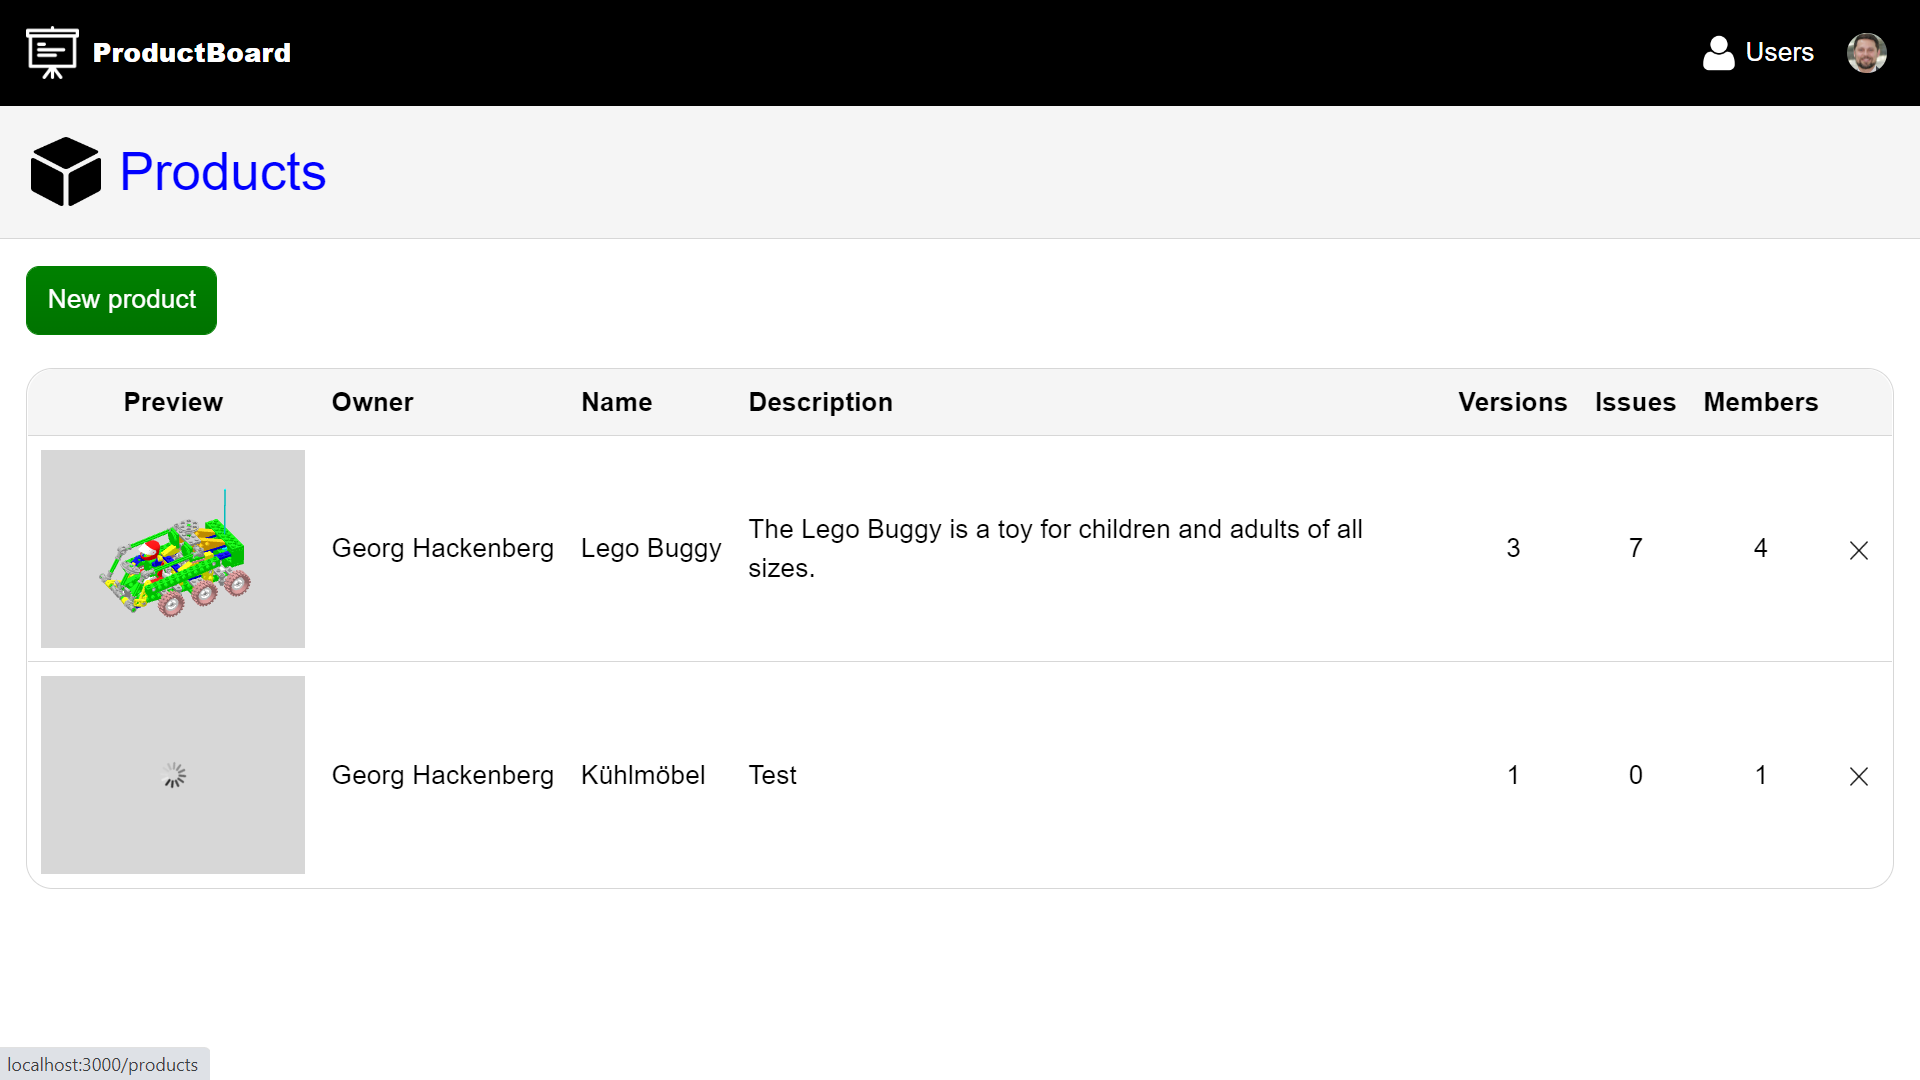
\includegraphics[width=0.5\textwidth]{screenshot-product.png}
    %\caption{Screenshot of the \textit{product overview}}
    \label{fig:screenshot-product}
\end{wrapfigure}

\subsubsection{Product overview}

The \textit{product overview} provides an overview of the products managed on the platform and visible to the current user.
On the top of the page, users with the product manager permission are provided a button to create a new product.
Then, for each product created previously a preview is shown of the latest CAD model revision that has been uploaded.
Furthermore, the name of the product owner is shown, i.e.\ the user with the product manager permission who has created the product originally.
Also, the human-readable name and description of the product are displayed to help the user navigate and distinguish different products.
Moreover, the number of CAD model revisions, the number of issues, and the number of members are listed for each product to provide an impression of user activity.
Additionally, users with product manager permission can see a cross button for each product, which allows them to delete the product from the database and from the list.
Finally, when clicking on the product, the user is redirected to the \textit{version overview} as introduced in the next section.

\begin{wrapfigure}{r}{0.5\textwidth}
    \centering
    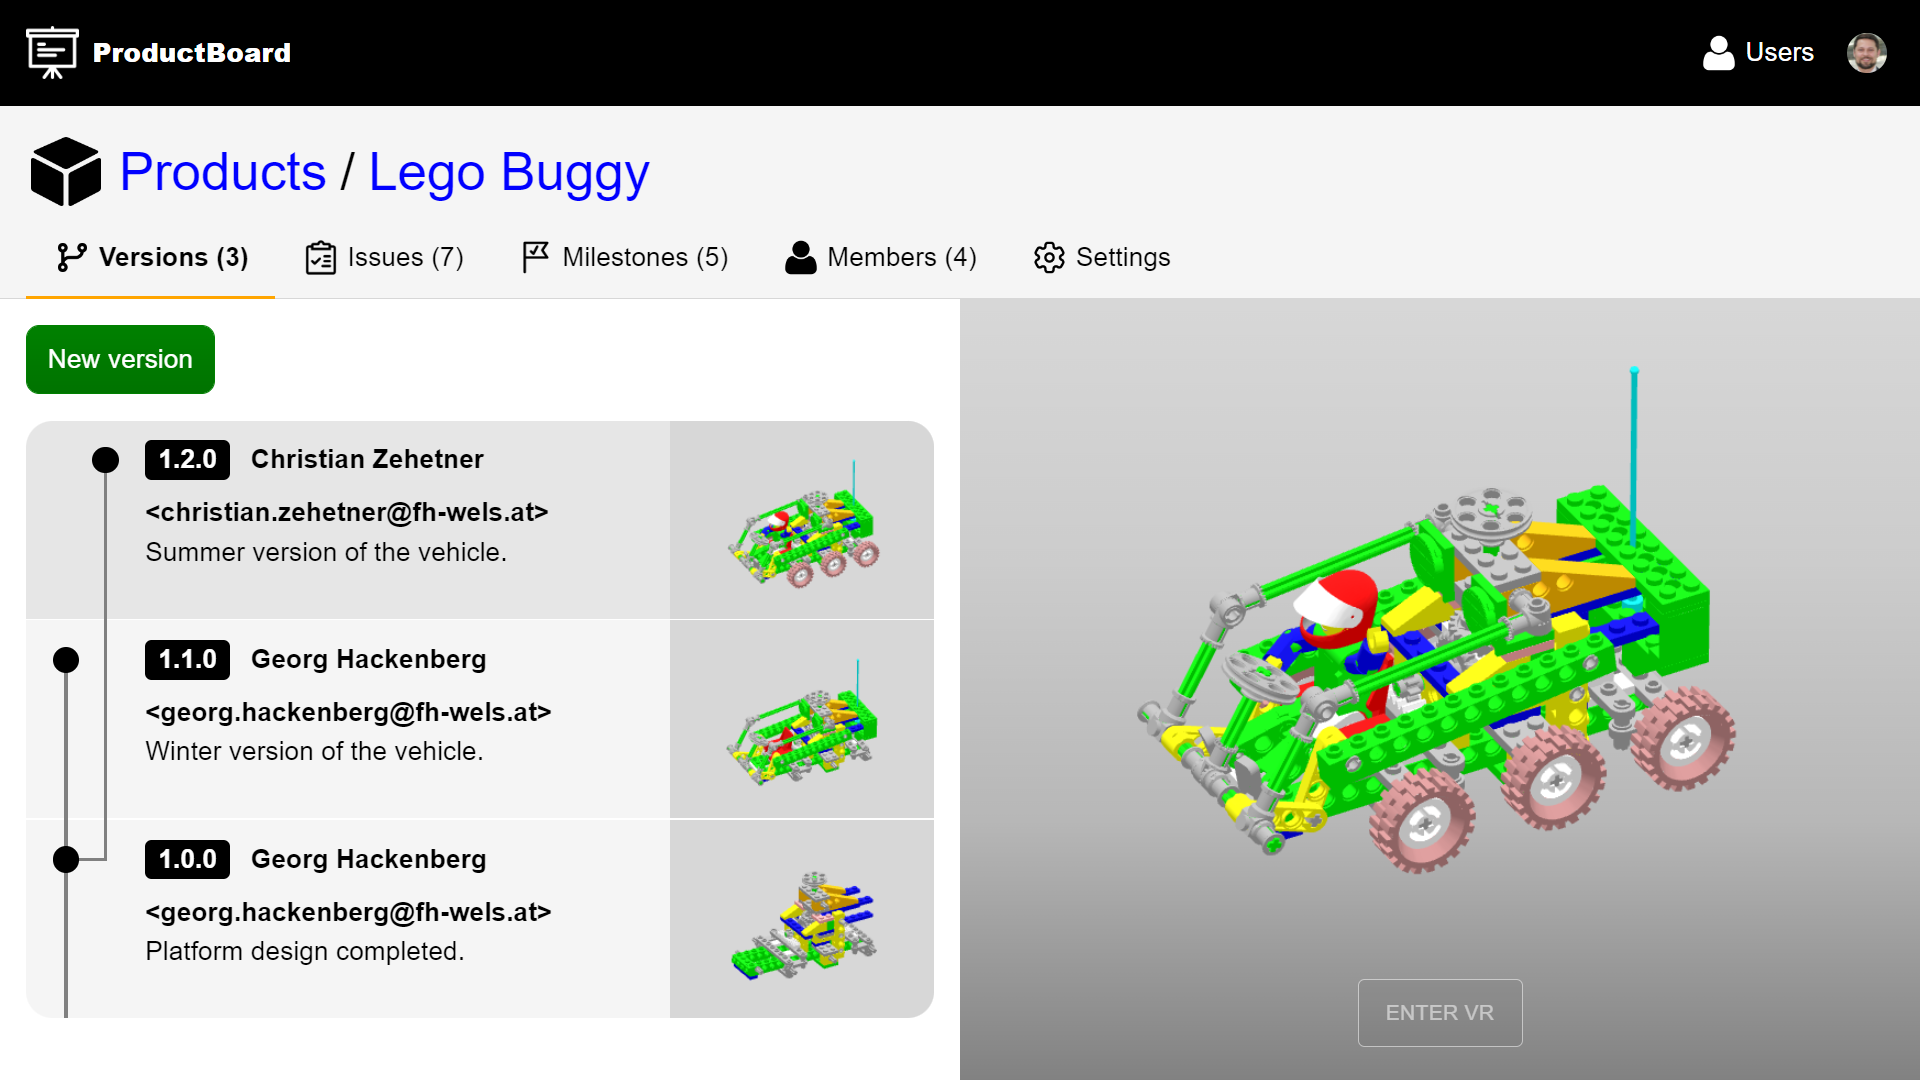
\includegraphics[width=0.5\textwidth]{screenshot-version.png}
    %\caption{Screenshot of the \textit{version overview}}
    \label{fig:screenshot-version}
\end{wrapfigure}

\subsubsection{Version overview}

The \textit{version overview} provides an overview of the CAD model revisions that have been uploaded for the selected product.
On the top of the page, users with the engineer member role are provided a button to create a new CAD model revision.
Then, for each CAD model revision the version number, the name of the user who created the version, a human-readable description of the changes that have been made, and links to respective base versions are displayed.
Note that for now the user selects the base versions manually when creating new CAD model revisions.
Furthermore, the user can select either none, one, or multiple base versions and, hence, describe \textit{branch} and \textit{merge} operations.
Additionally, previews of the different CAD model revisions are provided to help users understand the version history.
Finally, when clicking on a product version the associated CAD model revision is loaded into an interactive 3D view on the right side.
In this view the CAD model can be zoomed, rotated, and panned using mouse interactions or a virtual reality headset.

\begin{wrapfigure}{r}{0.5\textwidth}
    \centering
    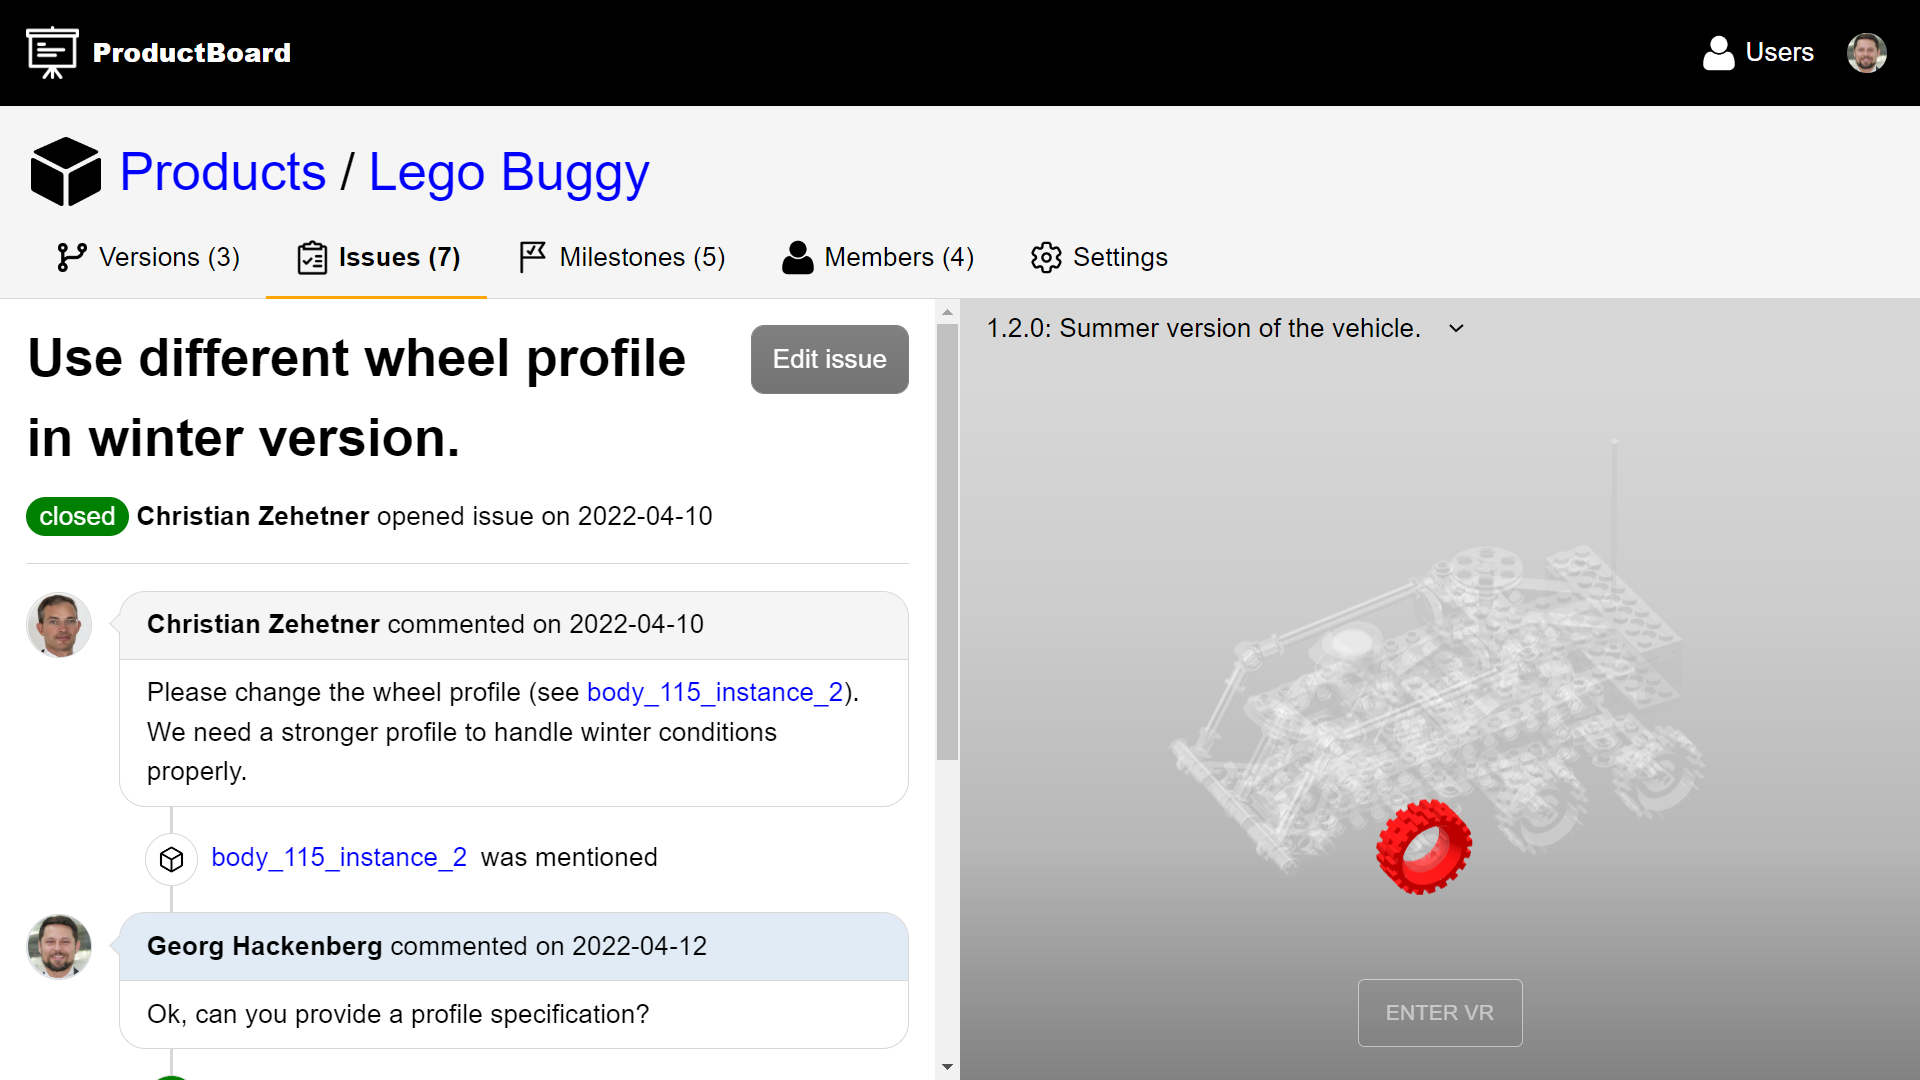
\includegraphics[width=0.5\textwidth]{screenshot-issue.png}
    %\caption{Screenshot of the \textit{issue detail view}}
    \label{fig:screenshot-issue}
\end{wrapfigure}

\subsubsection{Issue detail view}

Then, the \textit{issue detail view} provides an overview of the discussion between the different stakeholders around and open or closed design task.
On the top of the page the name of the issue is shown, which must be selected initially when creating the design task.
Below the name the state of the issue (open or closed), the name of the user who created the issue, and the date of creation are shown.
Afterwards, a list of comments is provided, which are attached to the issue.
For each comment the profile picture and the name of the user, who created the comment, as well as the date of creation are shown.
Furthermore, for each comment a human-readable description is shown, which can include markdown-based links to parts and assemblies of defined CAD model revisions.
Finally, on the right side a 3D view is provided which allows the user to select and display any CAD model revision of the product.
In this 3D view parts and assemblies are highlighted, which are referenced in the comments.
Additionally, new markdown-based references can be inserted into a comment field at the bottom of the page by mouse click onto the desired part or assembly.

\begin{wrapfigure}{r}{0.5\textwidth}
    \centering
    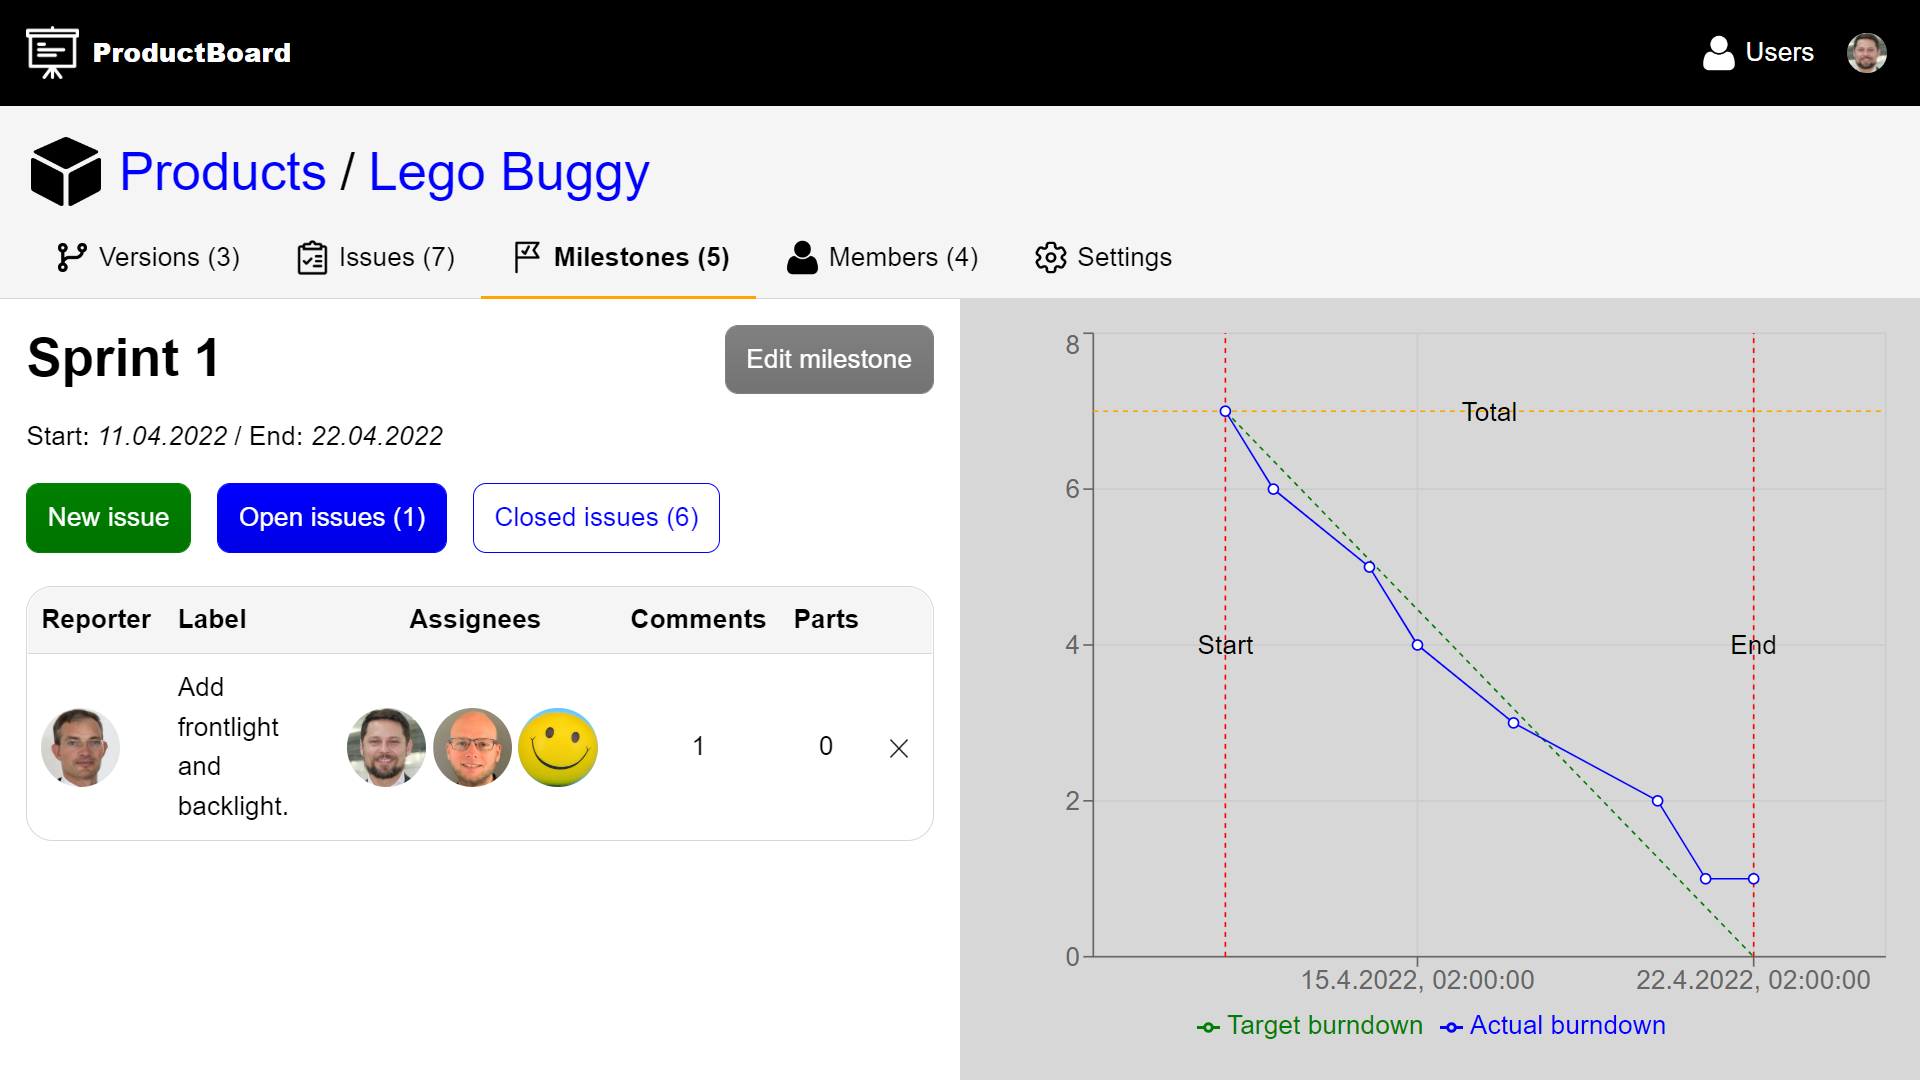
\includegraphics[width=0.5\textwidth]{screenshot-milestone.png}
    %\caption{Screenshot of the \textit{milestone detail view}}
    \label{fig:screenshot-milestone}
\end{wrapfigure}

\subsubsection{Milestone detail view}

The \textit{milestone detail view} provides an overview of the current sprint including open and closed design tasks.
At the top of the page the name of the milestone as well as the start date and the end date are shown.
Then, for users with the manager member role a button is provided, through which new milestones can be created.
Afterwards, the list of issues is displayed, which are assigned to the current milestone and which can be filtered by state (open or closed).
Furthermore, the list shows for each issue the profile pictures of the reporting and the assigned users, the name of the issue, as well as the number of comments and the number of referenced parts.
Finally, on the right side a burn down chart is being displayed, illustrating the progress of the current milestone.
The horizontal axis of the burn down chart shows the duration of the milestone from start date to end date.
The vertical axis of the charts shows the number of open issues instead.
Then, a target burn down line illustrates the ideal speed of issue resolution, while the actual burn down line shows the real speed.
This illustration helps the product manager to track progress.